\documentclass[a4paper,12pt]{article}

\usepackage{préambule}

\addtolength{\oddsidemargin}{-0.5cm}
\addtolength{\evensidemargin}{-0.5cm}
\addtolength{\textwidth}{1cm}

\makeatletter
\renewcommand{\maketitle}{%
{\tiny colle dans ton cahier d'exercices}
	\begin{center}
		\LARGE
		\uline{\@title}
		\vspace{1em}
	\end{center}
}
\makeatother

\title{Exercices symétrie centrale}
\date{}
\author{}

\begin{document}

\maketitle

\begin{exercice}[: Réflexion en groupe]\ \\
	\begin{enumerate}
		\item Imagine une personne devant un miroir.

		      Y-a-t'il une symétrie entre cette personne et son reflet ? Si oui, est-ce une symétrie axiale ou centrale ? \vspace{4em}
		\item Imagine deux jumeaux, qui s'habillent exactement pareil.

		      Y-a-t'il une symétrie entre ces deux personnes ? Si oui, est-ce une symétrie axiale ou centrale ? \vspace{4em}
	\end{enumerate}
\end{exercice}

\begin{exercice}
	Fait le symétrique des figures suivantes par rapport au point $O$ : \\

	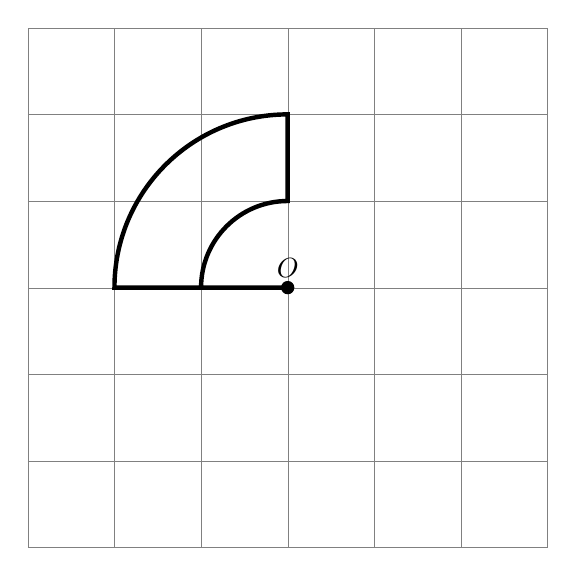
\begin{tikzpicture}[scale=1.1]
		\draw[step=1,gray,ultra thin] (0,0) grid (6,6);
		\coordinate (O) at (3,3);
		\filldraw[black] (O) node[anchor=south] {$O$} circle (2pt);

		\draw[ultra thick] (O) -- ++(-2,0) arc (180:90:2) -- ++(0,-1) arc (90:180:1);

		% \draw[ultra thick,rotate around={180:(O)}] (O) -- ++(-2,0) arc (180:90:2) -- ++(0,-1) arc (90:180:1);
	\end{tikzpicture} \hspace{1cm}
	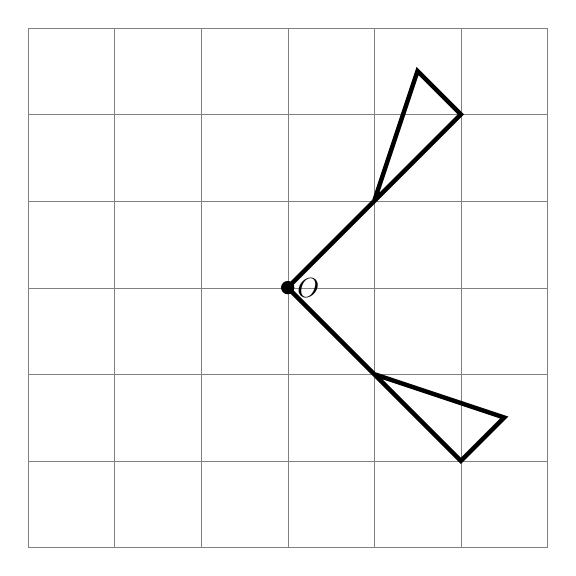
\begin{tikzpicture}[scale=1.1]
		\draw[step=1,gray,ultra thin] (0,0) grid (6,6);
		\coordinate (O) at (3,3);
		\filldraw[black] (O) node[anchor=west] {$O$} circle (2pt);

		\draw[black,ultra thick] (O) -- ++(2,-2) -- ++(0.5,0.5) -- ++(-1.5,0.5);
		\draw[black,ultra thick,rotate around={90:(O)}] (O) -- ++(2,-2) -- ++(0.5,0.5) -- ++(-1.5,0.5);
		% \draw[black,ultra thick,rotate around={180:(O)}] (O) -- ++(2,-2) -- ++(0.5,0.5) -- ++(-1.5,0.5);
		% \draw[black,ultra thick,rotate around={270:(O)}] (O) -- ++(2,-2) -- ++(0.5,0.5) -- ++(-1.5,0.5);
	\end{tikzpicture} \vspace{0.5cm}

	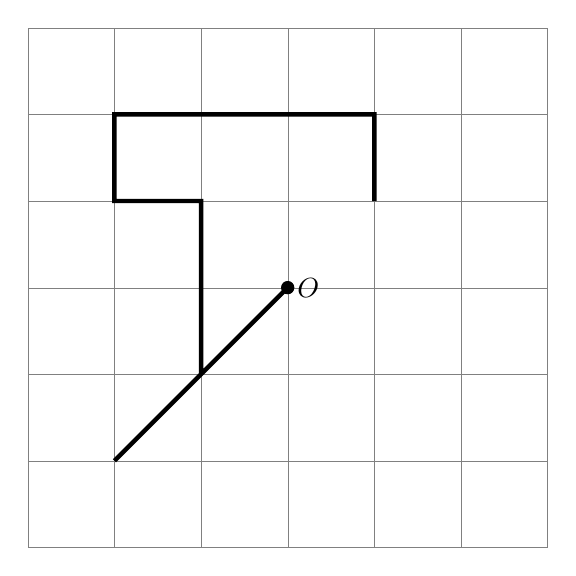
\begin{tikzpicture}[scale=1.1]
		\draw[step=1,gray,ultra thin] (0,0) grid (6,6);
		\coordinate (O) at (3,3);
		\filldraw[black] (O) node[anchor=west] {$O$} circle (2pt);

		\draw[ultra thick] (O) -- ++(-2,-2) ++(1,1) -- ++(0,2) -- ++(-1,0) -- ++(0,1) -- ++(3,0) -- ++(0,-1);

		% \draw[ultra thick,rotate around={180:(O)}] (O) -- ++(-2,-2) ++(1,1) -- ++(0,2) -- ++(-1,0) -- ++(0,1) -- ++(3,0) -- ++(0,-1);
	\end{tikzpicture} \hspace{1cm}
	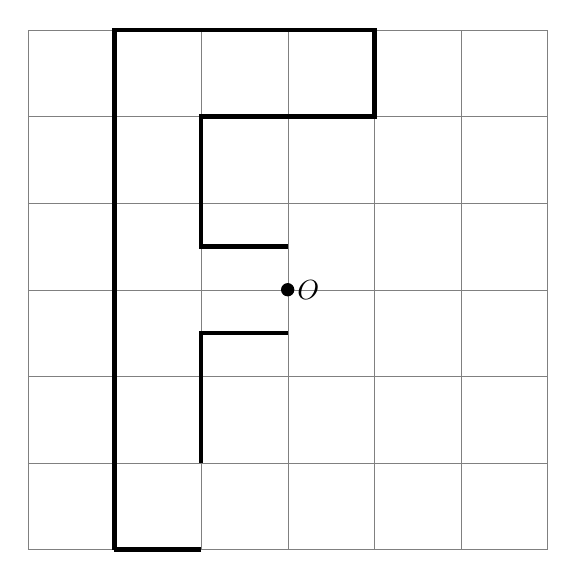
\begin{tikzpicture}[scale=1.1]
		\draw[step=1,gray,ultra thin] (0,0) grid (6,6);
		\coordinate (O) at (3,3);
		\filldraw[black] (O) node[anchor=west] {$O$} circle (2pt);

		\draw[ultra thick] (O) ++(-2,-3)-- ++(0,6) -- ++(3,0) -- ++(0,-1) -- ++(-2,0) -- ++(0,-1.5) -- ++(1,0) ++(0,-1) -- ++(-1,0) -- ++(0,-1.5) ++(0,-1) -- ++(-1,0);

		% \draw[ultra thick,rotate around={180:(O)}] (O) ++(-2,-3)-- ++(0,6) -- ++(3,0) -- ++(0,-1) -- ++(-2,0) -- ++(0,-1.5) -- ++(1,0) ++(0,-1) -- ++(-1,0) -- ++(0,-1.5) ++(0,-1) -- ++(-1,0);
	\end{tikzpicture}

	Appelle le professeur pour confirmer tes dessins.
\end{exercice}

\end{document}